\section{Motion in One Dimension and Changes in Velocity}

    \subsection{Position and Displacement}
        \textbf{Position-versus-time graph}: a graph that represents position ($x$) as a function of time ($t$).

        \begin{center}
            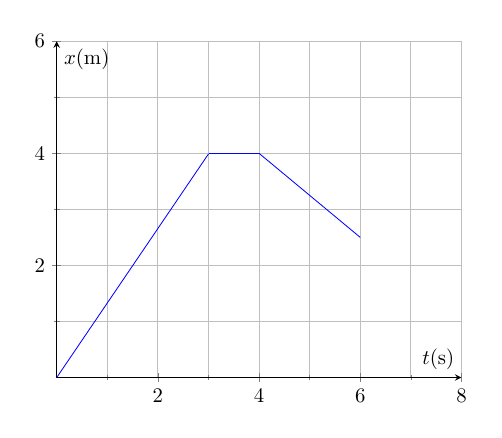
\begin{tikzpicture}[scale=0.75]
                \begin{axis}[
                    axis lines = middle,
                    smooth,
                    xlabel = $t$(s),
                    ylabel =$x$(m),
                    minor tick num =1,
                    grid=both,
                    no markers,
                    domain=0:8,
                    xtick={0,2,4,6,8},
                    ytick={0,2,4,6},
                    xticklabels={0,2,4,6,8},
                    yticklabels={0,2,4,6},
                    xmin=0,
                    xmax=8,
                    ymin=0,
                    ymax=6
                ]
                \addplot[
                    blue,
                    domain=0:3
                ]
                {1.33*x};
                \addplot[
                    blue,
                    domain=3:4
                ]
                {4};
                \addplot[
                    blue,
                    domain=4:6
                ]
                {-0.75*x+7};
                \end{axis}
            \end{tikzpicture}
        \end{center}

        \noindent Here, the object moves forward at a constant velocity between $t=0$ and $t=3$ as demonstrated by the even slope of the curve when $0\leq t\leq 3$. Then the object is at rest between $t=3$ and $t=4$,
        hence the curve is a flat line in that interval. Lastly, the object turns around and moves backward towards the origin, moving at a constant velocity again demonstrated by the even slope of the curve when
        $4\leq t \leq 6$. \\

        \noindent The \textbf{displacement} of an object is the vector change in position. The \textbf{$x$ component of displacement} is given by

        \[
            \Delta x = x_2 - x_1
        \]

        \noindent The particular wording of "$x$ component" reminds us that the $x$ component of displacement is measured along some specific $x$-axis. The $x$ component of displacement can be \textit{either} positive or
        negative. It is positive for displacements in the direction of increasing $x$ and negative for displacements in the direction of decreasing $x$. Whereas \textit{distance traveled} refers to the distance covered
        by a moving object along the path of its motion, \textit{displacement} describes a vector quantity with no reference position or axis. Only when motion is always in the same direction is the distance traveled
        equal to the distance between the initial and final positions.




    \subsection{Representing Motion}
        A curve in a position-versus-time graph is called an $\bm{x(t)}$ \textbf{curve} because it can be represented by a mathematical function $x(t)$.



    \subsection{Average Speed and Average Velocity}
        The slope of an $x(t)$ curve is the speed of the object at that time interval. Hence, in a position-versus-time graph, \textit{the steeper the slope, the higher the speed}.

        \[
            s_{avg} = \frac{\Delta x}{\Delta t}
        \]

        \noindent \textbf{Velocity} is a vector quantity expressing both speed and the direction of travel, where

        \begin{align*}
            x\text{ component of object's } v_{avg} &= \frac{x \text{ component of its displacement}}{\text{time interval for that displacement}} \\
            \Delta x \text{ of object's } v_{avg}   &= \frac{\Delta x \text{ of displacement}}{\Delta t \text{ for displacement}}
        \end{align*}

        \noindent A \textbf{velocity-versus-time graph} represents velocity ($v$) as a function of time ($t$). A curve plotted in such a graph is called a $\bm{v(t)}$ \text{curve}. We denote the $x$ component of an
        object's average velocity by $v_x$.




    \subsection{Scalars and Vectors}
        \textbf{Scalars} are physical quantities specified by a positive or negative magnitude and a unit of measurement. \\
        $\bullet$ e.g. temperature, volume, density, speed, energy, mass, time \\
        $\bullet$ written as a lowercase letter \\

        \noindent \textbf{Vectors} are physical quantities specified by a positive or negative magnitude, a unit of measurement, and a direction in space. \\
        $\bullet$ e.g. force, velocity, acceleration, displacement, momentum \\ \\
        $\bullet$ written as a lowercase letter with a right arrow over it, e.g. $\overrightarrow{v}$

        \noindent The \textbf{magnitude of a vector} is denoted by

        \[
            |\overrightarrow{b}| \text{ or } b
        \]

        \pagebreak

        \noindent To describe vectors mathematically, we use a \textbf{unit vector}, a vector whose sole purpose is to define a direction in space. Unit vectors do not have units and they have a magnitude of 1. Hence,

        \[
            |\hat{i}| = 1
        \]

        \noindent Unit vectors are denoted by a caret/hat ( $\hat{ }$ ) to distinguish them from normal vectors. Unit vectors pointing in the direction of increasing $x$ along the $x$-axis are denoted by
        $\hat{i}$ (pronounced \textit{$i$-hat}). \textbf{Unit vector notation} expresses a vector along the $x$-axis as the product of a scalar and the unit vector:

        \[
            \overrightarrow{b} = b_x \hat{i} \text{  (one dimension)}
        \]

        \noindent where $b_x$ is a scalar known as the $x$ component of $\overrightarrow{b}$. If we take the absolute value of both sides of the above equation, we find that, for vectors in one dimension, the magnitude
        of the vector $\overrightarrow{b}$ equals the magitude of $b_x$:

        \begin{align*}
            \overrightarrow{b}      &= b_x \hat{i} \\
            |\overrightarrow{b}|    &= |b_x \hat{i}| \\
                                    &= |b_x||\hat{i}| \\
                                    &= |b_x|
        \end{align*}

        \noindent If $b_x > 0$ then $\overrightarrow{b}$ is in the same direction as $\hat{i}$. If $b_x < 0$ then $\overrightarrow{b}$ is in the opposite direction to $\hat{i}$.



    \subsection{Position and Displacement Vectors}
        The most basic vector is displacement ($\Delta \overrightarrow{r}$). Recall that the $x$ component of displacement is equal to the change in the $x$ coordinate such that

        \[
            \Delta r_x = \Delta x = x_f - x_i
        \]

        \noindent The distance $d$ between two points is given by

        \[
            d = |x_1 - x_2 | \text{ (one dimension)}
        \]

        \noindent A vector that has zero magnitude is equal to the \textbf{zero vector}, denoted by a zero with an arrow ($\overrightarrow{0}$). In diagrams, the zero vector is represented by a dot. Rearranging the
        definition for $\Delta x$, we get

        \[
            x_f = x_i + \Delta x
        \]

        \noinent An object's position can also be represented by a vector:

        \[
            \Delta x \hat{i} = (x_f - x_i)\hat{i} = x_f \hat{i} - x_i \hat{i}
        \]

        \noindent where the left side of the equation represents the displacement

        \[
            \Delta x \hat{i} = \Delta r_x \hat{i} = \Delta \overrightarrow{r}
        \]

        \noindent The vector $x_i \hat{i}$ represents the \textbf{position vector}, a vector that lets us determine the position of a point in space relative to some chosen origin. Position is also represented by
        $\overrightarrow{r}$:

        \[
            \overrightarrow{r} = x \hat{i} \text{ one dimension}
        \]

        \noindent Hence, we can see that the $x$ component of position is equal to the coordinate such that

        \[
            r_x = x
        \]

        \noindent To subtract a vector from another vector, we reverse the direction of the vector being subtracted and add the reversed vector to the other vector:

        \begin{align*}
            \Delta \overrightarrow{r}  &= \overrightarrow{r_f} - \overrightarrow{r_i \\
                                        &= \overrightarrow{r_f} + (-1)\overrightarrow{r_i}
        \end{align*}

        \noindent The vector $\overrightarrow{a}-\overrightarrow{b}$ can be graphically represented like so:

        \begin{figure*}[hbt!]
            \centering
            \includegraphics[scale=0.75]{Resources/Vector_Subtraction}
        \end{figure*}

        \noindent Scalar multiplication of a vector:

        \[
            c\overrightarrow{a} = c\left(a_x \hat{i}\right) = \left(ca_x\right)\hat{i}
        \]



    \pagebreak
    \subsection{Velocity as a Vector}
        The $x$ component of the average velocity is given by

        \[
            v_{x,av} = \frac{\Delta x}{\Delta t} = \frac{x_f - x_i}{t_f - t_i}
        \]

        \noindent We can multiply the first and middle terms of the above equation by the unit vector $i$ and substitute $\Delta \overrightarrow{r} = \Delta x \hat{i}$ to get

        \[
            \overrightarrow{v_{av}} = v_{x,av}\hat{i} = \frac{\Delta \overrightarrow{r}}{\Delta t}
        \]

        \noindent Because $\Delta t$ is always positive, we see that for one dimensional motion, $\overrightarrow{v_{av}}$ always points in the same direction as displacement.



    \subsection{Motion at Constant Velocity}
        By convention, the phrase "average" is dropped from references to constant velocity. Thus, the $x$ component of the average velocity is simply $v_x$ and we see that the slope of the $x(t)$ curve is numerically
        equal to the $x$ component of the velocity:

        \[
            \frac{\Delta x}{\Delta t} = v_x \text{ constant velocity}
        \]

        \noindent The $x$ component of the displacement during any time interval is given by the area under the $v_x (t)$ curve between the beginning and the end of the time interval. We can use the fact that
        $\Delta x = x_f - x_i$ to rewrite the above equation in terms of $x_f$ such that

        \[
            x_f = x_i + v_x \Delta t \text{ constant velocity}
        \]



    \subsection{Instantaneous Velocity}
        \textbf{Instantaneous Velocity:} the velocity of an object at any given instant. The $x$ component of the velocity at instant $t$ is given by

        \[
            v_x = \lim_{\Delta t\to 0} \frac{\Delta x}{\Delta t} = \frac{dx}{dt}
        \]

        The velocity is then

        \[
            \overrightarrow{v} = v_x \hat{i} = \left(\lim_{\Delta t\to 0} \frac{\Delta x}{\Delta t}\right) \hat{i}
        \]

        Because the unit vector is constant, we can rewrite the velocity as

        \[
            \overrightarrow{v} = \lim_{\Delta t\to 0} \frac{\Delta x \hat{i}}{\Delta t} = \lim_{\Delta t\to 0}\frac{\Delta \overrightarrow{r}}{\Delta t} = \frac{d\overrightarrow{r}}{dt}
        \]

        Hence, speed is given by the magnitude of this vector:

        \[
            v = |\overrightarrow{v}|
        \]

hp

    \subsection{Changes in Velocity}
        \textbf{Acceleration}: the rate of change of velocity with respect to time. The $\bm{x}$ \textbf{component of average acceleration} is the change in the $x$ component of the velocity divided by the time interval
        during which this change took place. In physics, the word "\textit{deceleration}" has no meaning is better avoided, as \textit{acceleration} refers to \textit{any} change in velocity, regardless of increasing
        or decreasing speed. \\

        When an object's velocity and acceleration is in the same direction, the object speeds up. When they are in opposite directions, the object slows down. It is important to note confuse the positive $x$ component
        of acceleration with speeding up when working with objects traveling in the negative $x$ direction. An object speeds up when the magnitude of its velocity (aka speed) increases, regardless of the direction of
        motion. Whether or not the $x$ component of an object's acceleration is positive, however, dependson hte direction in which the object is moving. \\

        \begin{figure}[hbt!]
            \centering
            \caption*{\textbf{Position-versus-time graphs for objects accelerating along the positive $\bm{x}$ axis:}}
            \begin{subfigure}[b]{.45\textwidth}
                \includegraphics[scale=1]{Resources/Position_Time_Graph_Acceleration}
            \end{subfigure}
            \begin{subfigure}[b]{.45\textwidth}
                \includegraphics[scale=1]{Resources/Position_Time_Graph_Acceleration2}
            \end{subfigure}
        \end{figure}

        The curvature of an $x(t)$ curve is a measure of the $x$ component of acceleration. An upward curvature corresponds to a positive $x$ component of acceleration, whereas a downward curvature corresponds to a
        negative $x$ component of acceleration.



    \subsection{Acceleration Due to Gravity}
        In a vacuum, a feather and a stone drop at the same rate. Yet in air, the stone drops faster. This result has been attributed to air resistance pushing harder on the feather than the stone. \textbf{Free fall} is
        the motion of objects moving solely under the influence of gravity. A falling object inside a vacuum is in free fall because it is influenced only by gravity, but an object falling in the air is not in free fall
        because its motion is also affected by air resistance. However, the effect of air resistance on a stone outside of a vacuum is negligible. This property is true for many objects that are not too light and not
        dropped from too great of a height. Hence, if an object is not extremely light or dropped from a substantive height, we can ignore air resistance and consider all dropped objects to be in free fall. \\

        In the absence of air resistance, the \textbf{magnitude of the acceleration of all objects due to gravity} is $\bm{9.8}$ m/$\text{s}^2$ and consequently the amount of \textit{time it takes to fall from a certain height
        is the same for all falling objects.}



    \subsection{Projectile Motion}
        An object that is launched but not self-propelled is a \textbf{projectile}, and its motion is called \textbf{projectile motion}. The path a projectile follows is called its \textbf{trajectory}. The motion of an
        object in free fall is a special case of projectile motion. \\

        Consider a ball launched straight up. The ball slows down as it moves upward and hence its acceleration and velocity point in opposite directions. The ball's velocity changes \textbf{linearly}, changing by
        equal amounts in equal time intervals, thus its acceleration is constant. In the position-versus-time and velocity-versus-time graphs below, it can be seen that the slope of the $v_x (t)$ curve is about
        -10 m/$\text{s}^2$, which is the acceleration due to gravity. Thus, both on the way up and way down, the acceleration of a projectile is equal \textit{both in magnitude and in direction} to that of a freely falling
        object.

        \begin{figure*}[hbt!]
            \centering
            \caption*{$x(t)$ curve for a ball launched straight up:}
            \includegraphics[scale=0.8]{Resources/Projectile_Motion}
        \end{figure*}

        \begin{figure*}[hbt!]
            \centering
            \caption*{$v_x (t)$ curve for a ball launched straight up:}
            \includegraphics[scale=0.9]{Resources/Projectile_Motion2}
        \end{figure*}

        For an object launched upwards, the launch affects only the initial velocity. Once the object is released, the rest of its motion is determined by gravity alone (free fall). At the top of a trajectory of a ball
        launched upwards, there is instant at which the $x$ component of the velocity is zero. \textit{The $x$ component of the acceleration is not zero at the top}. To conceptualize this, consider the graph below.

        \begin{figure*}[hbt!]
            \centering
            \includegraphics[scale=0.6]{Resources/Nonzero_Acceleration_Trajectory}
        \end{figure*}

        Though velocity is zero at the apex of the trajectory, acceleration is defined as

        \[
            a = \frac{dv}{dt}
        \]

        The gradient of the line in the graph is nonzero and happens to be -9.81 m/$\text{s}^2$. Hence, the magntiude of the acceleration does not depend on $v$ and is equal to 9.81 m/$\text{s}^2$ for all values of $v$.



    \subsection{Motion Diagrams}
        \textbf{Motion diagrams} represent the positions of a moving object at equally spaced time intervals. We can make a motion diagrams by the following steps: \\

        1. Use dots to represent the moving object at even time intervals. If the object moves at constant speed then the dots are evenly spaced. Conversely, if the object speeds up, the spacing between the dots
        increases. If the object slows down, the spacing decreases. \\
        2. Choose an $x$ (position) axis convenient for the problem. This is usually an axis that has its origin at the initial or final position of the object and is oriented in the direction of motion or acceleration. \\
        3. Specify the position and velocity at all relevant interests, particularly, the \textbf{initial conditions}— position and velocity at the beginning of the time interval of interest, and the
        \textbf{final positions}— position and velocity at the end of that time interval. Additionally, specify all positions where the velocity reverses direction or the acceleration changes. Label any unknown
        parameters with a question mark. \\
        4. Indicate the acceleration of the object between all instants specified in step 3. \\
        5. To consider the motion of more than one object, draw separate diagrams side by side, one for each object, using one common $x$-axis. \\
        6. If the object reverses direction, separate the motion diagram into two parts, one for each direction of travel. \\

        An acronym for a useful checklist of a motion diagram is "\textbf{VENUS}": \\
        $\bullet$ \textbf{V}ectors and scalars used appropriately \\
        $\bullet$ \textbf{E}verything answered \\
        $\bullet$ \textbf{N}o unknowns left \\
        $\bullet$ \textbf{U}nits correct \\
        $\bullet$ \textbf{S}ignificant digits justified \\

        \begin{figure*}[hbt!]
            \centering
            \caption*{\textbf{A Motion Diagram:}}
            \includegraphics{Resources/Motion_Diagram}
        \end{figure*}




    \subsection{Summary of Symbols and Meanings in This Topic}

    \begin{center}
        \begin{tabular}{|c|c|}
            \hline
            \textbf{Symbol} & \textbf{Meaning} \\
            \hline
            $t$             & clock reading = instant in time \\
            \hline
            $\Delta t = t_f - t_i$  & change in clock reading = interval of time \\
            \hline
            $x$             & $x$-coordinate \\
            \hline
            $d=|x_1 - x_2|$ & straight-line distance between two points (never has sign) \\
            \hline
            $\hat{i}$       & unit vector defining direction of $x$-axis (vector magnitude 1) \\
            \hline
            $\overrightarrow{b} = v_x \hat{i}$  & vector and unit vector notation \\
            \hline
            $b_x$           & $x$ component of vector $\overrightarrow{b}$ (can be positive or negative) \\
            \hline
            $b=|\overrightarrow{b}|=|b_x|$  & magnitude of vector $\overrightarrow{b}$ (always positive) \\
            \hline
            $g=|\overrightarrow{a}_\text{free fall}|= 9.8$ m/$\text{s}^2$  & acceleration due to gravity near Earth's surface \\
            \hline
        \end{tabular}
    \end{center}

    \begin{center}
        \begin{tabular}{|c|c|c|c|}
            \hline
            \textbf{Vector} & \textbf{Meaning} & \textbf{Component} & \textbf{Meaning} \\
            \hline
            $\Delta \overrightarrow{r} = \Delta r_x \hat{i}$    & displacement & $\Delta r_x = \Delta x$    & $x$ component of displacement = change in $x$-coordinate \\
            \hline
            $\overrightarrow{r} = r_x \hat{i}$  & position & $r_x = x$  & $x$ component of position = $x$-coordinate \\
            \hline
            $\overrightarrow{v_{av}}=v_{x,av}\hat{i}$ & average velocity & $v_{x,av} = \frac{\Delta x}{\Delta t}$ & $x$ component of average velocity \\
            \hline
            $\overrightarrow{v} = v_x \hat{i}$ & (instantaneous) velocity   & $v_x = \lim_{\Delta t\to 0} \frac{\Delta x}{\Delta t} = \frac{dx}{dt}$ & $x$ component of (instantaneous) velocity \\
            \hline
            $\overrightarrow{a} = a_x \hat{i}$ & acceleration & $a_x = \frac{\Delta v_x}{\Delta t} = \frac{dv_x}{dt} = \frac{d^2 x}{dt^2}$ & $x$ component of acceleration \\
            \hline
        \end{tabular}
    \end{center}

    \textbf{Average Velocity}: The constant velocity required to achieve the same displacement in the same time interval as the actual motion.

    \[
        v_{avg} = \frac{1}{t_2 - t_1} \int^{t_2}_{t_1} v(t) dt
    \]

    Note that this is just the average value of a function integral.